\documentclass[10pt,a4paper,danish]{article}
%% Indlæs ofte brugte pakker
\usepackage{amssymb}
\usepackage[danish]{babel}
\usepackage[utf8]{inputenc}
\usepackage{listings}
\usepackage{fancyhdr}
\usepackage{hyperref}
\usepackage{booktabs}
\usepackage{graphicx}
\usepackage{todonotes}
\usepackage{algorithmic}
\usepackage{amsmath}

\pagestyle{fancy}
\fancyhead{}
\fancyfoot{}
\rhead{\today}
\rfoot{\thepage}
\setlength{\parindent}{0pt}

% Opsæt indlæsning af filer
\lstset{
 language=Python,
 extendedchars=\true,
 inputencoding=utf8,
 linewidth=\textwidth, basicstyle=\small,
 numbers=left, numberstyle=\footnotesize,
 tabsize=2, showstringspaces=false,
 breaklines=true, breakatwhitespace=false,
}

%% Titel og forfatter
\title{G3\\Maskinarkitektur\\Efterår 2011}
\author{Jens Fredskov\\ Naja Mottelson\\Søren Pilgård}

%% Start dokumentet
\begin{document}

%% Vis titel
\maketitle
\newpage

%% Vis indholdsfortegnelse
\tableofcontents
\newpage

%% Klar, parat, start!
\section{Indledning}
Denne rapport dokumenterer gruppens arbejde med tredje godkendelsesopgave i kurset 
Maskinarkitektur. Det udleverede afprøvningsprogram kører på vores besvarelsesarkitektur 
(NB! Mere om afprøvning!). 

\paragraph{}
I nærværende rapport har vi valgt at fokusere på at beskrive de punkter på 
hvilke vores implementering adskiller sig fra det man kan finde i lærebogen - 
de steder hvor vi har valgt at følge bogens tilgang er derfor højst meget 
kort beskrevet. 

\paragraph{}
Af overordnede afvigelser fra lærebogen kan nævnes vores valg mht. indeksering:
Imellem hver pipeline videresender vi PC + 4 i stedet for PC. Dette sparer os 
for at trække 4 fra PC'en ved Hopforudsigelsestabellen. 

\paragraph{}

\section{Fremsendingsenhed}
Vores implementering af kredsløbets fremsendingsenhhed (se \ref{fig:fu}) er 
en direkte oversættelse af den pseudokode der er at finde i lærebogen (s. 369)
- dog med de rettelser der er at finde i opgaveformuleringen. 

\paragraph{}
Ved undersøgelse for datafarer i MEM-stadiet undersøges der først 
for hvorvidt MEM/WB.RegWrite er sat, og at destinationsregistret
ikke er \$0. Hvis dette er tilfældet sammenlignes destinationsregistret
med hhv. rs- og rt-registrene i ID/EX (hvis en lighed findes har vi en 
datafare). Logikken for undersøgelse for EX-datafarer er implementeret
på samme vis, og ført igennem en NOT-gate for at lede til det endegyldige
udtryk. 

\begin{figure}[htb]
\begin{center}
\leavevmode
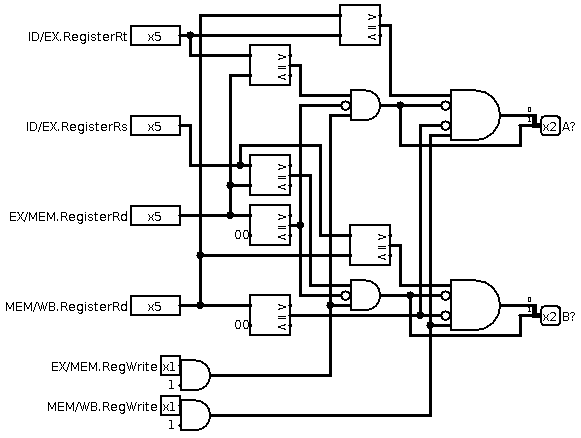
\includegraphics[scale=0.70]{forwarding_unit.png}
\end{center}
\caption{Fremsendingsenhed}
\label{fig:fu}
\end{figure}

\section{Fareafsløringsenhed}
Ligesom fremsendingsenheden er vores fareafsløringsenhed (se \ref{fig:hdu})
implementeret fra pseudokoden i COD (s. 372). Det er vigtigt at bemærke at 
det eneste enheden foretager sig er at stalle - informationen om hvorvidt de 
enkelte jump-instruktioner flusher pipeline-registre eller ej har vi flyttet
ud i hver enkelt pipeline, som så modtager en flush-bit fra instruktionen. 

Fareafsløringsenheden sammenligner rs- og rt-registrene i IF/ID og ID/EX. Hvis
to af dem er ens og ID/EX.MemRead-bitten er høj, sender fareafsløringsenheden
en stall-bit ud i systemet. Stall-bitten sendes til programtælleren, hvor den 
benyttes til at (disable) skrivning. Den sendes også til en or-gate hvis 
funktion er at flushe ID/EX-pipelinen. 

\begin{figure}[htb]
\begin{center}
\leavevmode
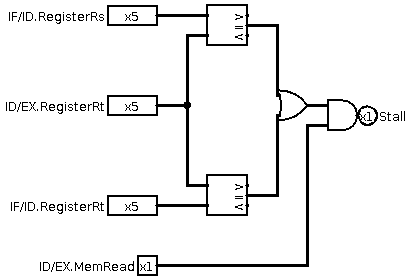
\includegraphics[scale=0.70]{hazard_detection_unit.png}
\end{center}
\caption{Fareafsløringsenhed}
\label{fig:hdu} 
\end{figure}

\section{Jump-instruktioner}

\subsection{Jump}
Når jump-bitten i kontrollen er sat (enten i IF/ID eller ID/EX) flusher vi 
instruktionerne i IF/ID, og sender jump-bitten til en MUX som vælger imellem
at sende JumpAddr og den sædvanlige inkrementerede værdi til programtælleren.
Denne mux modtager også input fra hopforudsigelsesenheden. 

\subsection{Jump and link}
Vi har ændret kontrollogikken for jal-instruktionen så vi, såfremt
jal-bitten er sat, allerede vælger register \$31 i afkodningsstadiet
 - vi sender \$31 med som instruktionens rd-felt i resten af kredsløbet,
hvor det bruges som signal til fremsendingsenheden. Såfremt jal-bitten 
er sat flusher vi også IF/ID. 

\subsection{Jump register og Branch on equal}
Logikken til håndtering af både jr- og beq-instruktionerne har vi 
placeret i en separat enhed ved navn Jump and Branch. Disse to 
instuktioners implementering er nærmere beskrevet under afsnittet
om hopforudsigelse. 

\section{Hopforudsigelse}

\subsection{Hopgætteenhed}

\subsection{Hopudførselsenheden}


\end{document}
